\section{Buildroot}
\subsection{Principaux répértoires}
\begin{figure}[H]
\centering
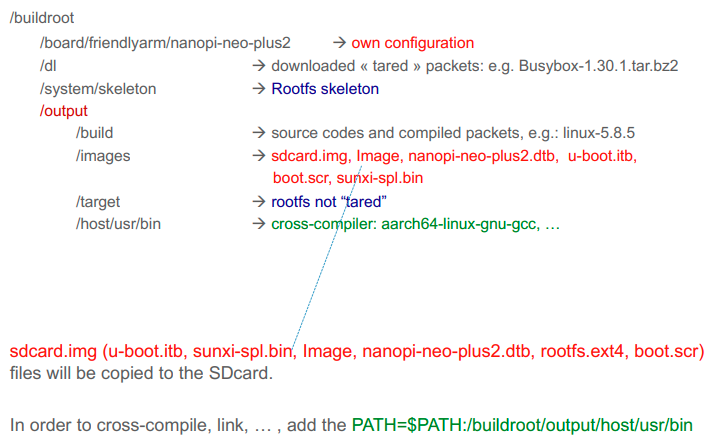
\includegraphics[width=0.9\columnwidth]{Figures/buildroot_01.png}
\end{figure}
Ce qui est manquant dans le répértoire dans le dossier output sera recompilé lors de la commande \verb! make! ou en précisant le paquet : \verb!make <package>-rebuild! à refaire.
\subsection{Principe de fonctionnement}
Basé sur des fichiers \verb!make! \verb!kconfig!, buildroot est un outil qui automatise le process de construction d'un système Linux embarqué en utilisant la cross-compilation. Lors de la commande \verb!make! il va s'occuper de compiler l'entier du système et préparer une image complète et prête pour l'utilisation.
\subsection{Configuration pour un hardware donné}
Il y a un répertoire situé dans \verb!board/friendlyarm/nanopi-neo-plus2! qui contient plusieurs fichiers intéressants. On y retrouve notamment le fichier \verb!nanopi-neo-plus2/nanopi-neo-plus2.dts! qui contient le FTD ("Flattened Device Tree") qui décrit le hardware. On indique donc à buildroot l'emplacement de ce fichier avec la commande \verb!menuconfig!. Autres fichiers intéressants : 
\begin{figure}[H]
\centering
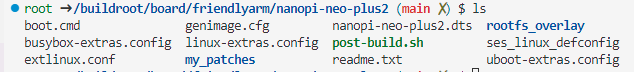
\includegraphics[width=0.9\columnwidth]{Figures/buildroot_02.png}
\end{figure}
\subsection{Patch buildroot}
Il faut spécifier le dossier des patchs \verb!make menuconfig! nous on a fait dans \verb!/nanopi-neo-plus2/my_patches! et un dossier par package à patcher. Ensuite la technique consiste à profiter de l'outil git et se mettre dans \verb!/buildroot/output/build/uboot-2020.07! et de faire:
\begin{figure}[H]
\centering
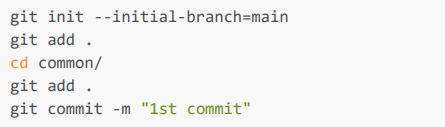
\includegraphics[width=0.9\columnwidth]{Figures/buildroot_03.png}
\end{figure}
Faire ensuite toutes les modifications à faire, les stager et faire la commande qui créé le patch au format voulu par buildroot:
\begin{Verbatim}[breaklines=true, breakanywhere=true]
git diff --cached --stat -p > /buildroot/board/friendlyarm/nanopi-neo-plus2/my_patches/uboot/0001_stack_protector.patch
\end{Verbatim}
On peut ensuite supprimer le paquet en question dans build et il se téléchargera et patchera automatiquement au prochain \verb!make!.
\subsection{Configuration de buildroot, u-boot, kernel}
Pour buildroot, on utilise \verb!make menuconfig! ça se sauvegarde dans \verb!.config! ou dans \verb!configs/ses_defconfig! (seulement les changement sont dans ce fichier, qui est à la base une copy de \verb!friendlyarm_nanopi_neo_plus2_defconfig! qui se situe au même endroit).\\
Pour u-boot, on va dans \verb!make menuconfig! catégorie bootloaders et ça va se sauver dans 
\begin{Verbatim}[breaklines=true, breakanywhere=true]
/buildroot/output/build/uboot-xx/configs/nanopi_neo_plus_defconfig
\end{Verbatim}
Et dans un fragment files qui ne contient que des petites modifications (save old, make new, use diff, add it to this fragment file): 
\begin{Verbatim}[breaklines=true, breakanywhere=true]
/buildroot/board/friedlyarm/nanopi-neo-plus/uboot-extras.config
\end{Verbatim}
Pour le kernel, \verb!make linux-menuconfig!, ça save dans \verb!/buildroot/output/build/linux-xx/defconfig! et nous on le copie et le met dans \verb!ses_linux_defconfig!
\subsection{Génération de la carte SD}
Pour créer le fichier \verb!sdcard.img! utilise le script \verb!genimage.sh! qui va aller aussi utiliser le fichier \verb!nanopi-neo-plus2/genimage.cfg! qui spécifie les différentes partitions à créer et les images (venant de \verb!output/images!) à mettre dedans.

\subsection{Génération du rootfs}
Il est copié depuis \verb!/buildroot/system/skeleton! pour le mettre dans \verb!/buildroot/output/target!. Il est ensuite possible d'ajouter des fichiers et des répértoires avec le \verb!/nanopi-neo-plus2/rootfs_overlay!. Après la commande \verb!make! le pseudo rootfs est créé et placé dans un des fichiers images de sorties \verb!rootfs.xxx!

\subsection{rootfs\_overlay}
On peut préprarer la structure des fichiers de la cible dans ce dossier

\subsection{Installer un nouveau package dans buildroot}
Pour utiliser un package, il faut faire \verb!make menuconfig! et aller choisir le package à aller utiliser. Sinon il faut ajouter le nouveau package "foo" dans le dossier \verb!/buildroot/package!. Il doit contenir au moins:
\begin{itemize}
\item Config.in: in kconfig language : on pourra y accéder à travers \verb!make menuconfig!
\item foo.mk: fichier qui décrit ou prendre les sources et comment les installer
\item optional foo.hash: pour vérifier l'intégrité des fichiers à télécharger
\item optional Sxx\_foo: le startup script pour le package foo
\end{itemize}